\chapter{Versuchsdurchführung}

In diesem Kapitel wird der Versuchsaufbau beschrieben sowie eine Versuchsanleitung gegeben.

\section{Versuchsaufbau}

Folgende Hardware sollte sich in Ihrer Versuchskiste befinden. Bitte überprüfen sie dies vor Beginn des Versuches.

\begin{itemize}
    \item RespberryPi 3 mit eingesetzter SD-Karte
    \item CC2531 Sniffer Stick
    \item cod.m ZigBee CC2652P2 Raspberry Pi Module
    \item 2 x Phillips Hue White E27
    \item 1 x Phillips Hue dimmer switch
    \item HDMI Kabel
    \item Ethernet Kabel
\end{itemize}

Das cod.m Modul sollte bereits auf Ihrem Raspberry montiert sein. 

\section{Aufgabenstellungen}

Bitte arbeiten sie die folgenden Aufgabenstellungen durch. Fertigen sie im Anschluss einen Versuchsbericht an.

\subsection{Aufgabe 1 - Vorbereitungen}

\subsubsection{Vorbereitung}
a) Schließen sie an den RaspberryPi Monitor, Tastatur ,Maus sowie den Sniffer-Stick an. Durch Anschluss der
Stromversorgung startet der Raspberry automatisch. Melden sie sich mit folgenden Zugangsdaten an:

\begin{itemize}
    \item User: student 
    \item Password: zigbeelab
\end{itemize}

b) Starten sie ein Konsolenfester und überprüfen mit folgendem Befehl, ob die Container ausgeführt werden:
\begin{lstlisting}
    > docker ps
\end{lstlisting}

Es sollten 3 Container im Status \grqq Running\grqq{} sein. 

\subsubsection{ZigBee2Mqtt Einrichtung}

c) Starten sie den Webbrowser Firefox und Navigieren zu der Seite:
\begin{lstlisting}
    https://z2m.local
\end{lstlisting}

d) Überprüfen Sie, dass keine Geräte mit dem Koordinator verbunden sind. Sollten Geräte in der Netzwerkübersicht ersichtlich sein, setzen sie den Versuch zurück.
Dies wird in den FAQs beschrieben.\\


e) Starten sie Wireshark über das Symbol auf dem Desktop. Bei den verfügbaren Schnittstellen sollte sich eine \grqq TI CC22531\grqq{} Schnittstelle finden. Über das vorangestelle Zahnrad-Symbol können sie den abzuhörenden
 Kanal einstellen. Stellen sie den eben gewählten Zigbee Kanal ein. (Gruppennummer)

Starten sie einen Capture Vorgang und warten einigen Sekunden ab.

Beenden sie den gestarteten Capture Vorgang. Gehen sie in das Menü: Bearbeiten > Einstellungen > Protokolle > ZigBee > Edit (Pre-configured Keys) und tragen
hier den \grqq TC-Link Key\grqq{} und den \grqq Network Key\grqq{} ein. Als \grqq Network Key\grqq{} verwenden sie den in Zigbee2Mqtt gesetzen Key. Der \grqq TC-Link Key\grqq{} ist ein
Standard-Key, der verwendet werden muss.
\begin{lstlisting}
    0x 5A 69 67 42 65 65 41 6C 6C 69 61 6E 63 65 30 39 (ZigBeeAlliance09)
\end{lstlisting}

\begin{Hinweis}
    Alle Aufgaben sollen mit Wireshark mitgeschnitten werden. Lesen sie die Aufgabenstellung erst durch und machen sie sich den Ablauf klar. Versuchen sie das 
    Zeitfenster des Wireshark Mitschnitts so kurz wie möglich zu halten, und in dieser Zeit nur die in der Aufgabenstellung explizit beschrieben Aktionen durchzuführen.
\end{Hinweis}

\subsection{Aufgabe 2 - Joining einer Phillips Hue Lampe}
a) Schalten sie eine der beiden Lampen ein. Setzen sie die zweite Lampe zurück, indem sie auf der Fernbedienung die beiden äußeren Tasten drücken während sie diese dicht an die Lampe halten. Die Lampe muss mehrmals blinken.\\\\
b) Starten sie nun ein Wireshark Mitschnitt und erlauben in zigbee2mqtt das Anlernen von Geräten. Sobald zigbee2mqtt ein erfolgreiches Interview gemeldet hat, beenden sie
den Capture Vorgang. Die Lampe signalisiert durch ein kurzes blinken einen erfolgreiches Interview.

\begin{figure}[H]
    \centering
    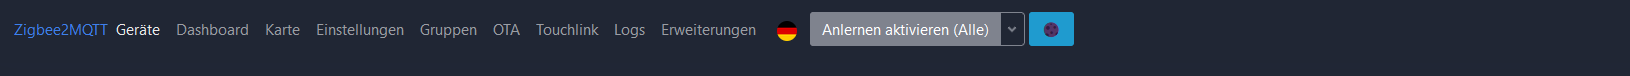
\includegraphics[width=1\textwidth]{media/Z2M-Anlernen.png}
    \caption{Zigbee Anlernen aktivieren}
\end{figure}

\begin{Aufgabe}
    Speichern sie den Wireshark Capture ab als \textbf{\grqq <Gruppe> - ZigbeeLab - Aufgabe 2.1\grqq{}}. \\
    Beantworten sie die Fragen in Ihrem Versuchsbericht.
\end{Aufgabe}

c) Navigieren sie nun zur Übersichtsseite der Lampe. Diese sollte ähnlich wie folgende Seite aussehen:

\begin{figure}[H]
    \centering
    \includegraphics[width=1\textwidth]{media/Z2M-Übersichtsseite.png}
    \caption{Zigbee Device Übersicht}
\end{figure}

d) Vergeben sie in der Übersichsseite der Lampe einen nutzerfreundlichen Namen. Dies geschieht über den blauen Button im unteren Teil der Übersicht.\\
e) Dimmen und schalten sie die Lampe über die Weboberfläche. Die ist unter dem Reiter \grqq Details\grqq{} möglich. Starten sie einen weiteren Capture Vorgang und
schneiden in diesem einen Schaltvorgang mit.

\begin{Aufgabe}
    Speichern sie den Wireshark Capture ab als \textbf{\grqq <Gruppe> - ZigbeeLab - Aufgabe 2.2\grqq{}}. \\
    Beantworten sie die Fragen in Ihrem Versuchsbericht.
\end{Aufgabe}

\subsection{Aufgabe 3 - Joining eines Gerätes über ein anderes Gerät}
Für diese Aufgabe sollte nur eine Lampe mit dem Koordinator verbunden sein. Die zweite Lampe wird nun über die Lampe dem Netzwerk hinzugefügt. Aus diesem Grund wird es nur der Lampe
erlaubt ein neues Gerät aufzunehmen. 

a) Setzen sie die zweite Lampe zurück, indem sie auf der Fernbedienung die beiden äußeren Tasten drücken während sie diese dicht an die Lampe halten. Die Lampe muss mehrmals blinken.\\
b) Erlauben sie den Beitritt neuer Geräte explizit für die bereits verbundene Phillips Lampe.
Ein erfolgreiches anlernen wird auch hier in der Weboberfläche und durch ein blinken der grünen LED signalisiert. 

\begin{figure}[H]
    \centering
    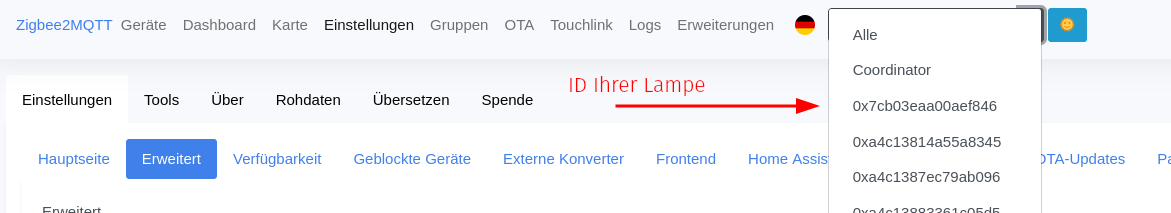
\includegraphics[width=1\textwidth]{media/Z2M-Anlernen-Lampe.png}
    \caption{Zigbee Anlernen aktivieren - nur Lampe}
\end{figure}

\begin{Aufgabe}
    Speichern sie den Wireshark Mitschnitt ab als \textbf{\grqq <Gruppe> - ZigbeeLab - Aufgabe 3\grqq{}}. \\
    Beantworten sie die Fragen in Ihrem Versuchsbericht.
\end{Aufgabe}

c) Sehen sie sich die Netzwerkübersicht unter dem Reiter \grqq Karte\grqq{}. Aktivieren sie nur den Haken \grqq isParent\grqq{} \\
d) Fügen sie die Fernbedienung Ihrem Netzwerk hinzu. Gehen sie dabei wie bisher vor. Die Fernbedienung lässt sich durch das drücken aller 4 Tasten gleichzeitig zurücksetzen. Drücken sie diese solange bis die LED Grün/Orange blinkt
Die Fernbedienung lässt nun zwar ein neues Netzwerk zu, allerdings sucht sie nicht auf neuen Kanälen. Bei einem Kanalwechsel kann es notwendig sein, die Batterie längere Zeit zu entfernen oder den \grqq Setup \grqq{} Knopf auf der
Rückseite zu betätigen.\\

Ihre Übersichtsseite sollte wie folgt aussehen.

\begin{figure}[H]
    \centering
    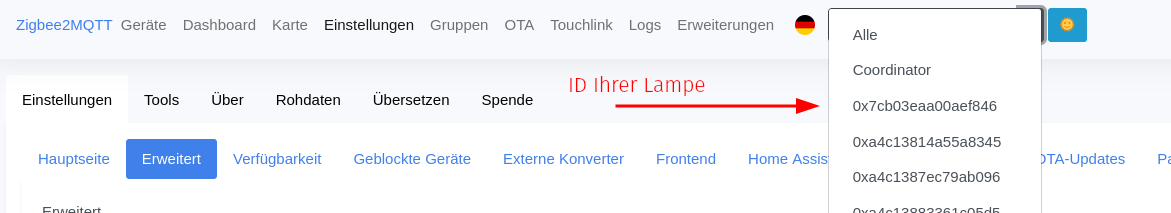
\includegraphics[width=1\textwidth]{media/Z2M-Anlernen-Lampe.png}
    \caption{Zigbee Anlernen aktivieren - nur Lampe}
\end{figure}


\subsection{Aufgabe 4 - Binding der Fernbedienung}

a) Navigieren sie in der Weboberfläche zu der Übersicht Ihrer Lampe. Dort finden sie einen Reiter \grqq binden\grqq{}. \\
b) Starten sie ein Wireshark Mitschnitt. Binden sie den Endpunkt X Ihrer Lampe mit dem Endpunkt X Ihrer Fernbedienung. \\
c) Schalten sie nun die Lampe mit der Fernbedienung ein und aus. 

\begin{Hinweis}
    Speichern sie den Wireshark Capture ab als \textbf{\grqq <Gruppe> - ZigbeeLab - Aufgabe 4\grqq{}}. \\
    Beantworten sie die Fragen in Ihrem Versuchsbericht.
\end{Hinweis}



\subsection{Aufgabe 5 - Gruppenbildung}

a) Navigieren sie in der Weboberfläche zu dem Reiter \grqq Groups \grqq{}. \\
b) Legen sie eine Gruppe mit dem Namen \grqq Hue-Lights-<Gruppe> \grqq{} an.\\
c) Starten sie einen Wireshark Mitschnitt. Editieren sie nun die Gruppe. Fügen sie die Endpunkte der beiden Lampen, die zum Steuern verwendet werden, der Gruppe hinzu. \\
d) Navigieren sie nun wieder zur Binding-Übersicht der Fernbedienung. Entfernen sie das Binding zu der Lampe. Binden sie die Fernbedienung nun mit der soeben
angelegten Gruppe.

\begin{figure}[H]
    \centering
    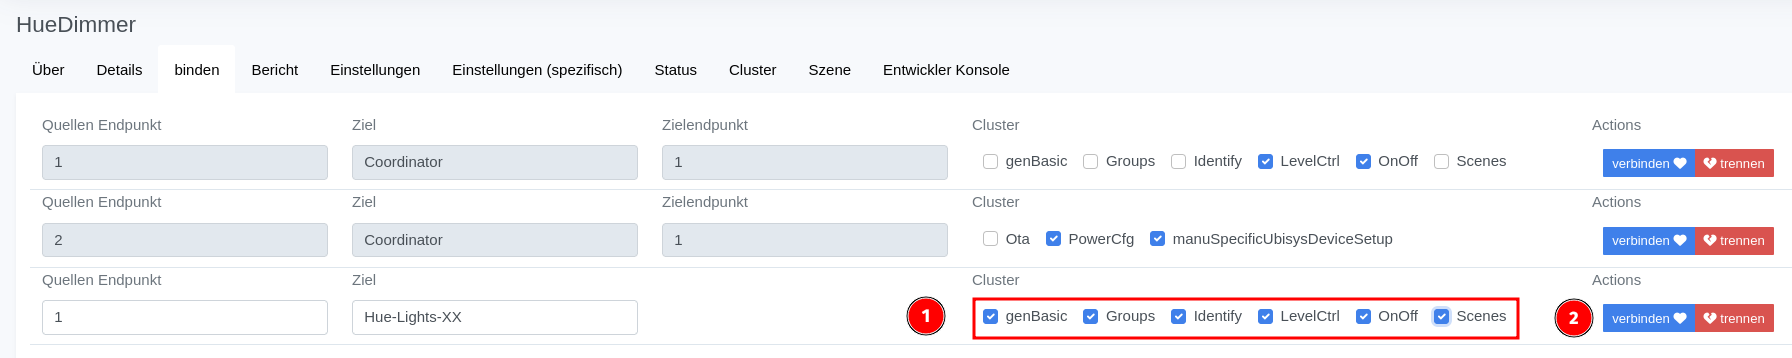
\includegraphics[width=1\textwidth]{media/Z2M-Group-Binding.png}
    \caption{Zigbee Group Binding}
\end{figure}

Achten sie darauf, alle hier genannten Cluster anzuwählen.

\begin{Aufgabe}
    Speichern sie den Wireshark Capture ab als \textbf{\grqq <Gruppe> - ZigbeeLab - Aufgabe 5\grqq{}}. \\
    Beantworten sie die Fragen in Ihrem Versuchsbericht.
\end{Aufgabe}


\subsection{Fragen}
\subsubsection{Aufgabe 2}

\begin{Fragen}
    1. Untersuchen sie den \textbf{Beacon-Request}\\
    Erläutern sie den Frametype und den Command Identifier.\\ 
    Erläutern die Ziel- und Quelladdresse und was sie daraus erschließen können.\\
    
    2. Wie teilt der Koordinator den umliegenden Geräten mit, dass er dem Netzwerk den Beitritt weiterer Geräte erlaubt ?\\
    Zu welchem Frametype gehört der Beacon und durch welchen Wert wird er spezifiziert?\\
    Welche Ziel- und Quelladressen werden verwendet?\\
    
    4. Welchen Wert hat das Feld „Association Permit“ im letzten Beacon des Koordinators und wie ist dieser Wert zu interpretieren? \\
    
    5. Untersuchen Sie den \textbf{Association Request} der Lampe an den Koordinator. \\
    Welchen Wert hat das Feld \grqq Allocate Address \grqq{} und wie ist dieser zu interpretieren?\\
    Welchen Wert hat das Feld \grqq Device Type\grqq{} und wie ist dieser zu interpretieren?\\
    
    7. Untersuchen die den "Data Request" von der Lampe an den Koordinator.\\
    Erläutern Sie die Funktion dieser Nachricht.\\
    Mit welchem Kommandoframe antwortet der Koordinator auf den Data-Request?\\
    Welche Werte besitzen die Felder „Short Address“ und „Association Status“?\\
    
    8. Untersuchen Sie einen \textbf{IEEE802.15.4. Ack-Frame}.\\
    Welche Adressfelder werden benutzt? \\
    Wie findet die Zuordnung zum Daten- oder Kommandoframe statt, der durch die Ack bestätigt wird? \\
    Werden grundsätzlich alle Frames bestätigt?\\
    
    10. Wie lautet die letzte Nachricht, bei der 64-bit-MAC-Adressen verwendet werden und wie\\
     lautet die erste Nachricht, bei der die 16-Bit-Kurzadresse der beigetretenen Lampe verwendet wird?\\
    
    11. Was ist die letzte Nachricht, die auf dem NWL-Layer unverschlüsselt übertragen wird?\\
    
    12. Erläutern Sie den Zweck der \textbf{Tranport-Key-Nachricht}.\\
     Wie lautet der Frametype des 802.15.4-Frames, in dem die Transport-Key-Nachricht transportiert wird? \\
     Wie lautet der ZigBee-NWK Frametype des Frames?\\
     Treffen Sie möglichst genaue Aussagen zum in der Transport-Key übertragenen Schlüssel (Schlüsseltype). \\
     Erläutern Sie, wie die Transport-Key-Nachricht kryptographisch gesichert ist.\\
     Interpretieren Sie den Inhalt des Radius Feldes im NWK-Frame, das die TransportKeyNachricht enthält!\\
    
    13. Erläutern Sie, den Zweck des versendeten \textbf{Active-Endpoint-Requests} und des \textbf{SimpleDescriptor-Requests}.
     Beschreiben Sie die Information, die in den entsprechenden Response-Nachrichten enthalten ist. 
     Wie stellt deConz die Information dar?
     Welche Endpoints werden für den Austausch der untersuchten Request- und ResponseNachrichten verwendet? Interpretieren Sie dies!

    14. Durch welche ZigBee-Frames werden die Schaltvorgänge übertragen? \\
    
    15. Beschreiben Sie möglichst genau, durch welche Headerfelder die Schaltvorgänge definiert sind! \\
        
    16. Welche Endpoints werden für die Schaltvorgänge benutzt? Woher hat der Koordinator Kenntnis über die in der Lampe verwendeten Endpoints? \\
    \end{Fragen}
    \subsubsection{Aufgabe 3}
    \begin{Fragen}
        1. Erläutern Sie den Zweck der \textbf{Permit-Join-Request} Nachricht. An welche ZigBee-NWKZieladresse wird die Nachricht versendet? 
        Erläutern Sie das wichtigste Headerfeld!\\
        
        2. Welchem Zweck dient die \textbf{Update Device} Nachricht? Wer ist Absender und wer ist
        Empfänger? Welche Adresse steht im Feld „Device Address“?\\
        
        3. Von welchem Device erhält die zweite Lampe ihre 16 Bit Kurzadresse und wie lautet sie?\\
        
        4. Wie viele \textbf{Transport-Key} Nachrichten wurden ausgetauscht? Erläutern Sie wer jeweils
        der Absender und wer der Empfänger ist. Versuchen Sie die den Vorgang zu erklären und
        gehen Sie dabei auf das Kommandoframe \grqq Tunnel\grqq{} ein. Wie sind die Transport-Key Nachrichten kryptographisch gesichert?
        Was sind die wichtigsten Headerfelder des Tunnel-Kommandoframes?\\
        
        5. Untersuchen Sie die \textbf{Device Announcement} Nachricht der zweiten Lampe, welchen
        Zweck hat sie? Schauen Sie sich die \grqq Capability Information \grqq{} an. Handelt es sich um ein
        Full-Function-Device? Welcher Wert steht im Feld „AC Power“ und was sagt dieser Wert aus? \\
        
        6. Untersuchen Sie die \textbf{Active-Endpoint-Request} Nachricht und ihren Weg vom
        Koordinator bis zur zweiten Lampe. Vergleichen Sie die Adressen im ZigBee-NWKLayer und im IEEE-Layer und erklären Sie den Zusammenhang. An welchem Headerfeld
        können Sie zweifelsfrei identifizieren, dass es die gleiche Nachricht ist, die nur weitergeleitet wird? \\
        
        7. Untersuchen Sie die \textbf{Simple Descriptor Response}- Nachrichten der zweiten Lampe!
        Welche Informationen enthält diese Nachricht? \\

        8. Erklären sie die Zahlen, welche in der Kartenansicht an den Verbindungen notiert sind.\\
        \end{Fragen}
        \subsubsection{Aufgabe 4}
        \begin{Fragen}
            1. Untersuchen Sie die \textbf{Bind Request}- und die \textbf{Bind Response}-Nachricht. 
            Was sind jeweils die NWK-Quell- und NWK-Zieladressen? Erläutern Sie, den Inhalt der BindRequest Nachricht. 
            Was genau bewirkt die Nachricht? In der Nachricht sind nur 64-Bit Adressen enthalten. Stellt das ein Problem dar? \\
            
            2. Warum wird vom Koordinator kein Bind-Request an die Lampe gesendet. \\
            
            3. Betrachten Sie die \textbf{ZCL: OnOff} Nachricht. Geben Sie die NWK-Quell- und Zieladresse an. 
            Welchen Wert hat das On/OFF-Cluster und welches Kommando wird zum Schalten verwendet?\\
            
            4. Interpretieren Sie die von der Fernbedienung gesendeten \textbf{Data Request} Nachrichten?
            Wie groß ist der zeitliche Abstand zwischen zwei Data-Requests? Was löst eine DataRequest-Nachricht beim Empfänger aus? Geben Sie ein Beispiel. 
            \end{Fragen}

            \subsubsection{Aufgabe 5}

            \begin{Fragen}
                1. Verdeutlichen Sie sich den Vorgang in dem Sie die vom Koordinator versendeten
                Nachrichten \textbf{Get Group Membership} bzw. \textbf{Add Group} untersuchen. Fassen Sie die
                wichtigsten Informationen der Nachrichten zusammen. \\
                
                2. Betrachten Sie die \textbf{Add Group Response} Nachricht des Empfängers.
                Welche Information ist enthalten? Welcher Zielendpunkt wird im APS-Frame des AddGroup-Befehles verwendet? Geben
                Sie eine Erklärung! \\
                
                3. Wie lautet die Destination Adresse im ZDP-Header der \textbf{Bind Request} Nachricht?
                Welcher Zielendpunkt ist vorhanden? \\
                
                4. Was ist die NWK-Zieladresse der \textbf{ZCL-OnOff} Nachricht? Um welche Art von Nachricht handelt es sich hierbei?
                Finden Sie die von Ihnen eingestellte Gruppen-ID in der „ZCL OnOff“-Nachricht wieder? \\
                \end{Fragen}
                
1. Welchem Zweck dienen die „Link Status“ Nachrichten? Über welche Anzahl von „Hops“
wird diese Nachricht übertragen? Analysieren Sie exemplarisch einige Link-StatusNachrichten und Interpretieren Sie diese! \\


2. Untersuchen Sie die „Link Quality Request“- bzw. „Link Quality Response“-Nachrichten.
Gehen Sie auf den LQI-Wert in der „Link Quality Response“ Nachricht und was bedeutet
dieser? \\


3. Interpretieren Sie „Route Request“ Nachrichten und zugehörige „Route-Response“-
Nachrichten. 




